Es bien sabido que, en principio, una descripción correcta de los sistemas físicos requiere el uso de la Mecánica Cuántica, por lo que una formulación correcta de la Mecánica Estadística solo puede hacerse dentro del marco de las ideas mecánico-cuánticas, a pesar de que, en muchos casos, la Mecánica Clásica proporciona una excelente aproximación al problema, como hemos visto hasta ahora.

Así, aunque el esquema general de la Mecánica Estadística desarrollado en los capítulos anteriores sigue siendo válido cuando la descripción mecánica de las partículas que componen el modelo microscópico se realiza mediante la Mecánica Cuántica, la aplicación de los postulados y las leyes cuánticas tiene importantes implicaciones en las propiedades finales de los sistemas. Además: corno analizaremos seguidamente, la Mecánica Estadística Cuántica no solo recupera los resultados obtenidos con la Clásica, sino que también soluciona las dificultades conceptuales anteriormente encontradas.

De entre los resultados que se derivan de tina descripción cuántica de los sistemas físicos, los que se deducen de la indistinguibilidad de las partículas y las propiedades de simetría de las funciones de onda jugarán un papel esencial en lo que sigue, por lo que comenzaremos este capítulo con una breve recopilación de los mismos.

\newpage
\section{Función de particion de un gas cuántico ideal}

En este apartado y los siguientes vamos a considerar el modelo microscópico de un gas ideal cuando la descripción del mismo se realiza mediante la Mecánica Cuántica.
Como veremos, aparecen hechos peculiares que son consecuencia de la indistinguibilidad cuántica de las partículas.

Así, pues, consideremos un sistema de $N$ partículas idénticas cuyas fuerzas de interacción pueden despreciarse. Vamos a utilizar la siguiente nomenclatura:

\begin{itemize}
	\item Las propiedades que se refieran a una partícula las representaremos mediante letras minúsculas, de forma que escribiremos $r$ para el estado cuántico de una partícula, $\varepsilon_r$ para la energía de ese estado y $n_r$ para el número de partículas que se encuentran en el mismo estado $r$.
	
	\item Utilizaremos letras mayúsculas para las propiedades del sistema total.
	Así por ejemplo $E_R$ representa la energía del sistema total cuando se encuentra en el estado cuántico $R$.
\end{itemize}

Con esta notación son evidentes las relaciones
\begin{equation} \label{eq:E_R}
	E_R = \sum_r n_{r,R} \varepsilon_r
\end{equation}
y
\begin{equation}\label{eq:N_R}
	N_R = \sum_r n_{r,R}
\end{equation}
donde $n_{r,R}$ representa el número de partículas en el estado $r$, cuando el sistema se encuentra en el estado $R$.

Un estado cuántico $R$ de un sistema de partículas idénticas queda totalmente determinado si se conoce el número de partículas que se encuentran en cada estado $r$, no siendo posible especificar cuáles son las partículas que se encuentran concretamente en cada estado.
En consecuencia, un estado $R$ se puede especificar mediante el conjunto de números $\{n_r,R\}$ que se denominan \emph{números de ocupación}.

Como sabemos, las propiedades termodinámicas de cualquier sistema pueden determinarse evaluando su función de partición $Z$, definida como
\begin{equation}
	Z = \sum_R e^{-\beta E_R}
\end{equation}
que, utilizando \eqref{eq:E_R}, y teniendo en cuenta lo que acabamos de decir sobre la especificación de los estados, podrá escribirse
\begin{equation}\label{eq:Z_cuant}
	Z = \sum_{\substack{n_1, n_2, \ldots\\(\sum n_r =N)}} e^{-\beta (n_1 \varepsilon_1 + n_2 \varepsilon_2 + \cdots)} = \sum_{\substack{n_1, n_2, \ldots\\(\sum n_r =N)}} \exp \left[ -\beta \sum_r n_{r,R} \varepsilon_r \right] 
\end{equation}
ya que la suma sobre todos los estados $R$ se transformará en una suma extendida a todos los valores posibles de los números de ocupación, con la restricción de que su suma sea $N$ |número de partículas del sistema|, puesto que en la función de partición la suma se extiende sobre todos los estados accesibles a un sistema cerrado, esto es, con un número constante de partículas.

Sin embargo, el cálculo de la función de partición es bastante complicado, debido precisamente a la presencia de la condición restrictiva $\sum n_r =N$ Y resulta mucho más cómoda la utilización del \emph{conjunto canónico generalizado}, donde no existe dicha restricción.
Recordemos que las distintas colectividades son equivalentes en lo que se refiere a valores medios y propiedades termodinámicas, y que las diferencias aparecen en el problema específico de las fluctuaciones.

Así, pues, pasamos a considerar la gran función de partición que viene dada por
\begin{equation}
	Q = \sum_{N=0}^\infty e^{-\alpha N} \sum_{R}^{} {}^{(N)} e^{-\beta E_R} = \sum_{N=0}^\infty e^{-\alpha N_R -\beta E_R}
\end{equation}
donde, en la última expresión, el sumatorio respecto de $R$ se extiende sobre todos los estados posibles con cualquier número de partículas.
Utilizando \eqref{eq:E_R} y  \eqref{eq:N_R} podemos escribir
\begin{equation}
	Q = \sum_{N=0}^\infty \exp \left[ -\alpha \sum_r n_{r,R} -\beta \sum_r n_{r,R} \varepsilon_r \right] 
\end{equation}
o
\begin{equation}\label{eq:Q_cuant}
	Q = \sum_R \prod_r \exp \left[ -\alpha n_{r,R} -\beta n_{r,R} \varepsilon_r \right]  = \sum_R \prod_r \exp \left[  -(\alpha  + \beta \varepsilon_r) n_{r,R}\right]
\end{equation}

En esta expresión la suma para todos los estados $R$ equivale a sumar para todos los valores posibles del conjunto de números $\{n_r,R\}$ como en \eqref{eq:Z_cuant}, pero ahora sin restricción para la suma.
Dicho de otro modo, cada $n_r$ toma valores en \eqref{eq:Q_cuant} con independencia de cuáles sean los valores de los restantes números de ocupación, de manera que tenemos
\begin{equation}
	Q = \sum_{n_1, n_2, \ldots} \prod_r \exp \left[  -(\alpha  + \beta \varepsilon_r) n_r\right] = \sum_{n_1} \sum_{n_2} \cdots \prod_r \exp \left[  -(\alpha  + \beta \varepsilon_r) n_{r}\right]
\end{equation}

Es fácil ver ahora que esta expresión puede escribirse también en la forma
\begin{equation}\label{eq:Q_cuant2}
	Q = \prod_r \sum_{n=0}^{n_{max}} \exp \left[  -(\alpha  + \beta \varepsilon_r) n \right]
\end{equation}
donde $n_{max}$ representa el valor máximo que pueden tomar los números de ocupación.

\colorbox{red!60}{\textcolor{white}{\textit{[Aquí falta alguna cosilla, a saber si la hago]}}}

Ahora vamos a estudiar algunas propiedades formales de la gran función de partición en Mecánica Cuántica.

\subsection*{Número medio de partículas en un estado de partícula $\bm{r}$}
A partir de la definición general de valor medio tenemos
$$\expval{n_r} = \frac{\sum_R e^{-\alpha N_R -\beta E_R}}{Q} = \frac{1}{Q} \sum_R e^{-\alpha \sum_r n_{r,R} -\beta \sum_r n_{r,R} \varepsilon_r} = - \frac{1}{\beta} \frac{1}{q} \frac{\partial Q}{\partial \varepsilon_r}$$
o sea
\begin{equation}
	\expval{n_r} = - \frac{1}{\beta} \frac{\partial \ln Q}{\partial \varepsilon_r}
\end{equation}

\subsection*{Cálculo de la presión}

La expresión puede deducirse ---a gusto del lector ;)---, obteniéndose
\begin{equation}
	\left\langle p \right\rangle = \frac{1}{\beta} \left( \frac{\partial \ln Q}{\partial V} \right)_{\alpha, \beta}
\end{equation}

Si ahora utilizamos la expresión de $Q$, \eqref{eq:Q_cuant}, resulta
\begin{align*}
	\left\langle p \right\rangle &= \frac{1}{\beta Q} \sum_R \left\lbrace \left[ -\beta \sum_r n_{r,R} \left( \frac{\partial \varepsilon_r}{\partial V} \right) \right] \exp \left( -\alpha \sum_r n_{r,R} -\beta \sum_r n_{r,R} \varepsilon_r \right)  \right\rbrace \\
	&= \frac{1}{Q} \sum_R  \sum_r \left( \frac{\partial \varepsilon_r}{\partial V} \right) \sum_R n_{r,R} \exp \left( -\alpha \sum_r n_{r,R} -\beta \sum_r n_{r,R} \varepsilon_r \right)
\end{align*}
que, teniendo en cuenta la expresión de $n_r$, puede escribirse
\begin{equation}\label{eq:p_cuant}
	\left\langle p \right\rangle = \sum_r \left( \frac{\partial \varepsilon_r}{\partial V} \right) \expval{n_r} 
\end{equation}

Esta relación toma una forma especialmente útil en el caso particular de un sistema de partículas ideales encerradas en un volumen $V = L_xL_yL_z$, de forma que la energía de las partículas sea únicamente de traslación, y cuyos niveles energéticos vienen dados por
\begin{equation}\label{eq:e_r_gen}
	\varepsilon_r \equiv \frac{\hbar^2 \pi^2}{2m} \left[\left( \frac{n_x}{L_x} \right)^2 + \left( \frac{n_y}{L_y} \right)^2 + \left( \frac{n_z}{L_z} \right)^2 \right] 
\end{equation}
donde $n_x$, $n_y$ y $n_z$ son números cuánticos que pueden tomar valores enteros positivos |y que evidentemente no tienen nada que ver con los números de ocupación|.
Como las propiedades termodinámicas de un sistema deben ser independientes de la forma de éste) vamos a particularizar \eqref{eq:e_r_gen} al caso concreto de un cubo $(L_x = L_y = L_z = L)$ que es la forma más sencilla, obteniendo,
\begin{equation}
\varepsilon_r \equiv \frac{\hbar^2 \pi^2}{2mV^{2/3}} \left[ n_x^2 + n_y^2 + n_z^2 \right] 
\end{equation}
donde $V = L^3$.
En esta expresión aparece explícita toda la dependencia respecto del volumen, por lo que podemos calcular
$$\frac{\partial \varepsilon_r}{\partial V} = - \frac{2}{3 V} \varepsilon_r$$
que sustituida en \eqref{eq:p_cuant} da
\begin{equation}\label{eq:pv_t6}
	\left\langle p \right\rangle = \sum_r \frac{2}{3 V} \varepsilon_r \expval{n_r} = \frac{2}{3} \frac{\left\langle E \right\rangle}{V}
\end{equation}

Esta relación es válida independientemente de que las partículas que se consideren sean fermiones o bosones, con la condición de que los niveles energéticos de una partícula vengan dados por una expresión del tipo \eqref{eq:e_r_gen}.
En este sentido no será aplicable a gases poliatómicos ni a los fotones y fonones.
 
\section{Estadísticas de Fermi-Dirac y Bose-Einstein}
\subsection*{Estadística de Fermi-Dirac}

Vamos ahora a particularizar los resultados obtenidos en el apartado anterior para el caso de que las partículas que componen el sistema sean fermiones.
Sabemos que $n_r$ solo puede tomar entonces los valores 0 ó 1, de modo que $n_{max} = 1$ y \eqref{eq:Q_cuant2} toma la forma
\begin{equation}
	Q_{FD} = \prod_r \sum_{n=0}^{n=1} e^{-(\beta\varepsilon_r + \alpha) n} = \prod_r \left[ 1 + e^{ -( \beta\varepsilon_r + \alpha)} \right]
\end{equation}
de donde
\begin{equation}
	\ln Q_{FD} = \sum_r \ln \left[ 1 + e^{ -( \beta\varepsilon_r + \alpha)} \right]
\end{equation}

A partir de esta expresión obtenemos para el número medio de partículas en el sistema
\begin{equation}
	\expval{N} = - \frac{\partial \ln Q_{FD}}{\partial \alpha} = - \sum_r \frac{-e^{-\beta\varepsilon_r - \alpha}}{1 + e^{-\beta\varepsilon_r - \alpha}} = - \sum_r \frac{1}{1 + e^{\beta\varepsilon_r + \alpha}}
\end{equation}
y para el número medio de partículas en el estado r
\begin{equation}\label{eq:n_r_1}
	\expval{n_r} = - \frac{1}{\beta} \frac{\partial \ln Q_{FD}}{\partial \varepsilon_r} = \frac{1}{e^{\beta\varepsilon_r + \alpha} + 1}
\end{equation}
cumpliéndose, como es lógico, que $\expval{N} = \sum n_r$.
Además, como evidentemente se tiene
$$0 \leq e^{\beta\varepsilon_r + \alpha} \leq \infty$$
resulta que
$$0 \leq \expval{n_r} \leq 1$$
de acuerdo con el principio de exclusión de Pauli.

Esta expresión puede escribirse equivalentemente en función del potencial químico $\mu (T)$ ---que sabemos que está relacionado con $\alpha$ por $\alpha = -\beta\mu$--- en la forma
\begin{equation}\label{eq:n_r_2}
	\expval{n_r} = \sum_r \frac{1}{e^{\beta(\varepsilon_r - \mu)} + 1}
\end{equation}

Es usual en la bibliografía referirse a \eqref{eq:n_r_1} y \eqref{eq:n_r_2} como la \emph{distribución de Fermi}, reflejando el hecho de que indica el modo de distribuirse en valor medio las partículas entre los distintos estados.
Además, $\mu (T)$ recibe el nombre de \emph{nivel de Fermi} y su valor para $T = 0$, que representaremos por $\mu_0$, el de \emph{energía de Fermi} ---recordemos que el potencial químico tiene dimensiones de energía, como es fácil de comprobar---.
Así pues, escribiremos a partir de ahora
$$\mu_0 \equiv \mu(T=0)$$

\begin{wrapfigure}{r}{0.4\textwidth}
	\centering
	\hspace{3.5cm}
	% This file was created by matplotlib2tikz v0.6.15.

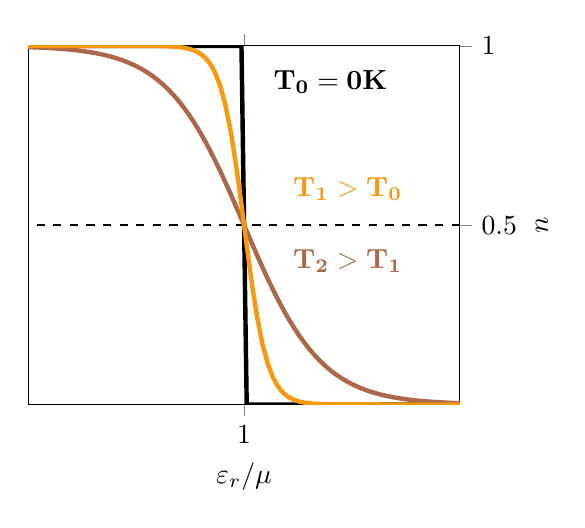
\begin{tikzpicture}

\definecolor{color0}{rgb}{0.12156862745098,0.466666666666667,0.705882352941177}
\definecolor{color1}{rgb}{1,0.498039215686275,0.0549019607843137}
\definecolor{color2}{rgb}{0.172549019607843,0.627450980392157,0.172549019607843}

\begin{axis}[
scale = 0.8,
xmin=-1.5, xmax=3.5,
ymin=0, ymax=1,
tick align=outside,
ytick pos=right,
yticklabel pos=right,
xtick = {1},
ytick = {0.5,1},
ylabel = {$\expval{n}$},
xlabel = {$\varepsilon_r/\mu$}]

\node at (2,0.9) {$\mathbf{T_0 = 0K}$};
\node at (2.2,0.6) {$\color{YellowOrange}\mathbf{T_1 > T_0}$};
\node at (2.2,0.4) {$\color{Sepia!50}\mathbf{T_2 > T_1}$};


\addplot [thick, black, dashed, forget plot]
table {%
	3.5 0.5
	-1.5 0.5
};

\addplot [ultra thick, black, forget plot]
table {%
-2 1
-1.93939393939394 1
-1.87878787878788 1
-1.81818181818182 1
-1.75757575757576 1
-1.6969696969697 1
-1.63636363636364 1
-1.57575757575758 1
-1.51515151515152 1
-1.45454545454545 1
-1.39393939393939 1
-1.33333333333333 1
-1.27272727272727 1
-1.21212121212121 1
-1.15151515151515 1
-1.09090909090909 1
-1.03030303030303 1
-0.96969696969697 1
-0.909090909090909 1
-0.848484848484848 1
-0.787878787878788 1
-0.727272727272727 1
-0.666666666666667 1
-0.606060606060606 1
-0.545454545454545 1
-0.484848484848485 1
-0.424242424242424 1
-0.363636363636364 1
-0.303030303030303 1
-0.242424242424242 1
-0.181818181818182 1
-0.121212121212121 1
-0.0606060606060606 1
0 1
0.0606060606060606 1
0.121212121212121 1
0.181818181818182 1
0.242424242424243 1
0.303030303030303 1
0.363636363636364 1
0.424242424242424 1
0.484848484848485 1
0.545454545454545 1
0.606060606060606 1
0.666666666666667 1
0.727272727272728 1
0.787878787878788 1
0.848484848484849 1
0.909090909090909 1
0.96969696969697 1
1.03030303030303 0
1.09090909090909 0
1.15151515151515 0
1.21212121212121 0
1.27272727272727 0
1.33333333333333 0
1.39393939393939 0
1.45454545454545 0
1.51515151515152 0
1.57575757575758 0
1.63636363636364 0
1.6969696969697 0
1.75757575757576 0
1.81818181818182 0
1.87878787878788 0
1.93939393939394 0
2 0
2.06060606060606 0
2.12121212121212 0
2.18181818181818 0
2.24242424242424 0
2.3030303030303 0
2.36363636363636 0
2.42424242424242 0
2.48484848484849 0
2.54545454545455 0
2.60606060606061 0
2.66666666666667 0
2.72727272727273 0
2.78787878787879 0
2.84848484848485 0
2.90909090909091 0
2.96969696969697 0
3.03030303030303 0
3.09090909090909 0
3.15151515151515 0
3.21212121212121 0
3.27272727272727 0
3.33333333333333 0
3.39393939393939 0
3.45454545454546 0
3.51515151515152 0
3.57575757575758 0
3.63636363636364 0
3.6969696969697 0
3.75757575757576 0
3.81818181818182 0
3.87878787878788 0
3.93939393939394 0
4 0
};
\addplot [ultra thick, Sepia!50, forget plot]
table {%
-2 0.998830489734944
-1.93939393939394 0.998659854927081
-1.87878787878788 0.998464362301224
-1.81818181818182 0.998240402586158
-1.75757575757576 0.997983846203057
-1.6969696969697 0.997689969430504
-1.63636363636364 0.997353370459146
-1.57575757575758 0.996967874067486
-1.51515151515152 0.996526423528682
-1.45454545454545 0.996020958237794
-1.39393939393939 0.995442275435552
-1.33333333333333 0.994779874306442
-1.27272727272727 0.994021780656891
-1.21212121212121 0.993154350348758
-1.15151515151515 0.9921620496943
-1.09090909090909 0.991027211138002
-1.03030303030303 0.989729762792429
-0.96969696969697 0.988246930803832
-0.909090909090909 0.986552914154096
-0.848484848484848 0.98461853242776
-0.787878787878788 0.982410848370265
-0.727272727272727 0.979892768836217
-0.666666666666667 0.977022630089974
-0.606060606060606 0.973753776504461
-0.545454545454545 0.970034145644023
-0.484848484848485 0.965805877646433
-0.424242424242424 0.961004972848204
-0.363636363636364 0.955561028785873
-0.303030303030303 0.949397096020685
-0.242424242424242 0.942429701491781
-0.181818181818182 0.934569097895778
-0.121212121212121 0.925719807196669
-0.0606060606060606 0.915781534655735
0 0.904650535100891
0.0606060606060606 0.892221513334469
0.121212121212121 0.878390132875692
0.181818181818182 0.863056188531365
0.242424242424243 0.846127465432218
0.303030303030303 0.827524257579285
0.363636363636364 0.807184451484523
0.424242424242424 0.785068996596897
0.484848484848485 0.761167489044236
0.545454545454545 0.73550349858496
0.606060606060606 0.708139185140206
0.666666666666667 0.679178699175393
0.727272727272728 0.648769858868011
0.787878787878788 0.617103662552354
0.848484848484849 0.584411335070708
0.909090909090909 0.550958815914465
0.96969696969697 0.517038854261009
1.03030303030303 0.482961145738991
1.09090909090909 0.449041184085535
1.15151515151515 0.415588664929292
1.21212121212121 0.382896337447646
1.27272727272727 0.351230141131988
1.33333333333333 0.320821300824607
1.39393939393939 0.291860814859794
1.45454545454545 0.26449650141504
1.51515151515152 0.238832510955764
1.57575757575758 0.214931003403103
1.63636363636364 0.192815548515476
1.6969696969697 0.172475742420715
1.75757575757576 0.153872534567782
1.81818181818182 0.136943811468635
1.87878787878788 0.121609867124308
1.93939393939394 0.107778486665531
2 0.0953494648991095
2.06060606060606 0.0842184653442654
2.12121212121212 0.0742801928033306
2.18181818181818 0.0654309021042215
2.24242424242424 0.0575702985082191
2.3030303030303 0.0506029039793152
2.36363636363636 0.0444389712141273
2.42424242424242 0.0389950271517962
2.48484848484849 0.0341941223535668
2.54545454545455 0.0299658543559764
2.60606060606061 0.0262462234955384
2.66666666666667 0.0229773699100256
2.72727272727273 0.0201072311637834
2.78787878787879 0.0175891516297347
2.84848484848485 0.0153814675722404
2.90909090909091 0.013447085845904
2.96969696969697 0.0117530691961683
3.03030303030303 0.0102702372075714
3.09090909090909 0.00897278886199761
3.15151515151515 0.00783795030569963
3.21212121212121 0.00684564965124238
3.27272727272727 0.00597821934310928
3.33333333333333 0.00522012569355839
3.39393939393939 0.00455772456444758
3.45454545454546 0.00397904176220586
3.51515151515152 0.00347357647131785
3.57575757575758 0.00303212593251372
3.63636363636364 0.00264662954085364
3.6969696969697 0.00231003056949582
3.75757575757576 0.00201615379694347
3.81818181818182 0.00175959741384183
3.87878787878788 0.00153563769877638
3.93939393939394 0.00134014507291926
4 0.00116951026505551
};
\addplot [ultra thick, YellowOrange, forget plot]
table {%
-2 0.99999999983081
-1.93939393939394 0.999999999733449
-1.87878787878788 0.99999999958006
-1.81818181818182 0.999999999338402
-1.75757575757576 0.999999998957681
-1.6969696969697 0.999999998357872
-1.63636363636364 0.999999997412897
-1.57575757575758 0.999999995924131
-1.51515151515152 0.999999993578643
-1.45454545454545 0.999999989883428
-1.39393939393939 0.999999984061774
-1.33333333333333 0.999999974890009
-1.27272727272727 0.999999960440287
-1.21212121212121 0.999999937675371
-1.15151515151515 0.999999901810223
-1.09090909090909 0.999999845306228
-1.03030303030303 0.999999756286619
-0.96969696969697 0.999999616040077
-0.909090909090909 0.999999395087745
-0.848484848484848 0.999999046987023
-0.787878787878788 0.99999849856976
-0.727272727272727 0.999997634563106
-0.666666666666667 0.999996273360716
-0.606060606060606 0.999994128852259
-0.545454545454545 0.999990750289837
-0.484848484848485 0.999985427555986
-0.424242424242424 0.999977041932086
-0.363636363636364 0.999963831026667
-0.303030303030303 0.999943018520036
-0.242424242424242 0.999910231066187
-0.181818181818182 0.999858580201049
-0.121212121212121 0.999777217303468
-0.0606060606060606 0.999649060409353
0 0.999447221363076
0.0606060606060606 0.999129397908724
0.121212121212121 0.998629090568688
0.181818181818182 0.997841893527604
0.242424242424243 0.996604213048194
0.303030303030303 0.994660517366896
0.363636363636364 0.991613642441852
0.424242424242424 0.986851109813223
0.484848484848485 0.979440056876836
0.545454545454545 0.967987443808298
0.606060606060606 0.95047788015511
0.666666666666667 0.924141819978756
0.727272727272728 0.885487519467777
0.787878787878788 0.830743967346632
0.848484848484849 0.757011372822882
0.909090909090909 0.664144375862977
0.96969696969697 0.556574869897311
1.03030303030303 0.443425130102689
1.09090909090909 0.335855624137023
1.15151515151515 0.242988627177118
1.21212121212121 0.169256032653367
1.27272727272727 0.114512480532223
1.33333333333333 0.0758581800212435
1.39393939393939 0.0495221198448899
1.45454545454545 0.0320125561917019
1.51515151515152 0.020559943123164
1.57575757575758 0.0131488901867773
1.63636363636364 0.00838635755814738
1.6969696969697 0.00533948263310347
1.75757575757576 0.00339578695180564
1.81818181818182 0.00215810647239593
1.87878787878788 0.00137090943131169
1.93939393939394 0.000870602091276129
2 0.0005527786369236
2.06060606060606 0.000350939590646793
2.12121212121212 0.000222782696532081
2.18181818181818 0.000141419798950703
2.24242424242424 8.97689338125817e-05
2.3030303030303 5.69814799643932e-05
2.36363636363636 3.61689733327415e-05
2.42424242424242 2.29580679137978e-05
2.48484848484849 1.45724440142074e-05
2.54545454545455 9.24971016298655e-06
2.60606060606061 5.8711477412452e-06
2.66666666666667 3.72663928418655e-06
2.72727272727273 2.36543689377272e-06
2.78787878787879 1.50143024043019e-06
2.84848484848485 9.53012976748569e-07
2.90909090909091 6.04912254635526e-07
2.96969696969697 3.83959923117318e-07
3.03030303030303 2.4371338079604e-07
3.09090909090909 1.54693772345089e-07
3.15151515151515 9.81897766388001e-08
3.21212121212121 6.23246294355404e-08
3.27272727272727 3.95597130002686e-08
3.33333333333333 2.51099909269281e-08
3.39393939393939 1.59382258667629e-08
3.45454545454546 1.01165724698257e-08
3.51515151515152 6.42135700517529e-09
3.57575757575758 4.07586915976196e-09
3.63636363636364 2.58710259838804e-09
3.6969696969697 1.64212824028369e-09
3.75757575757576 1.04231859930357e-09
3.81818181818182 6.61597575368682e-10
3.87878787878788 4.19940075870571e-10
3.93939393939394 2.66551259968483e-10
4 1.69189792232888e-10
};
\end{axis}

\end{tikzpicture}
	\vspace{-0.5cm}
\end{wrapfigure}
En la figura adyacente se representa la forma de $\expval{n_r}$ para distintos valores de la temperatura.
En el cero absoluto $(T = 0K)$, $\expval{n_r}$ es una función escalón y vale 1 para $\varepsilon_r \leq \mu_0$ y 0 para $\varepsilon_r > \mu_0$ de forma que todos los estados que correspondan a una energía menor o igual que la energía de Fermi están ocupados, mientras que los estados de energía superior están vacíos.
A temperaturas superiores, los niveles con energía inferior a $\mu$, pero próxima a él, comienzan a despoblarse en beneficio de los que poseen una energía superior.
Desde luego, en rigor, las curvas de la figura solo poseen significado para ciertos valores de $\varepsilon_r$ pues, como sabemos, los posibles valores de la energía de una partícula localizada en una cierta región del espacio tienen espectro discreto.

Obsérvese que para cualquier temperatura $T > 0 K$,
\begin{equation}
	\expval{n_r} (\varepsilon_r = \mu )= \frac{1}{2}
\end{equation}
y, por lo tanto, los estados con energía menor que la del nivel de Fermi, siempre tienen $\expval{n_r} > \sfrac{1}{2}$ y los que poseen una energía superior, $\expval{n_r} < \sfrac{1}{2}$.

\subsection*{Estadística de Bose-Einstein}

En el caso de bosones no existe limite para el número de partículas idénticas que pueden encontrarse en un mismo estado, de manera que $n_{max} = \infty$ y
\begin{equation}
	Q_{BE} = \prod_r \sum_{n=0}^{\infty} e^{-(\beta\varepsilon_r + \alpha) n}
\end{equation}

En esta expresión se observa que la suma se extiende ---para un $\varepsilon_r$ dado--- a los términos de una progresión geométrica indefinida de razón
$$e^{-(\beta\varepsilon_r + \alpha)} = e^{-\beta(\varepsilon_r - \mu)}$$
	
Esta serie es decreciente y, por lo tanto, su suma converge si la tazón es menor que la unidad o sea si
$$e^{-\beta(\varepsilon_r - \mu)} < 1$$
lo que equivale a
\begin{equation}\label{eq:cond_FD}
	\varepsilon_r - \mu > 0
\end{equation}

Esta condición se satisface siempre en las aplicaciones prácticas, para todos los estados $r$, ya que en otro caso el número de bosones en el sistema no estaría acotado.

Sumando la serie,\footnote{Recordemos que si $r < 1$ se tiene $\sum_{n=0}^{\infty} ar^n = \frac{a}{1-r}$} obtenemos
\begin{equation}
	Q_{BE} = \prod_r \frac{1}{1 - e^{-\beta\varepsilon_r + \alpha}}
\end{equation}
y, por lo tanto,
\begin{equation}\label{eq:Q_BE}
	\ln Q_{BE} = - \sum_r \ln (1 - e^{-\beta\varepsilon_r + \alpha})
\end{equation}

A partir de esta expresión deducimos
\begin{equation}
	\expval{N} = - \frac{\partial \ln Q_{BE}}{\partial \alpha} = \sum_r \frac{1}{e^{-\beta\varepsilon_r + \alpha} - 1}
\end{equation}
\begin{equation}\label{eq:n_r_BE}
	\expval{n_r} = \frac{1}{e^{-\beta\varepsilon_r + \alpha} - 1} = \frac{1}{e^{-\beta(\varepsilon_r - \mu)} - 1}
\end{equation}

Como es lógico, $\expval{n_r}$ puede ahora ser mayor que 1, y en particular tiende a infinito cuando $\varepsilon_r \rightarrow \mu$.
En la figura se representa el comportamiento de la función de distribución de Bose para distintos valores de la temperatura.
En el cero absoluto todos los bosones se agrupan en el estado de mínima energía, tendiendo a pasar a ocupar estados de mayor energía cuando se aumenta la temperatura.

Las expresiones correspondientes a ambas estadísticas pueden agruparse escribiendo
\begin{equation}
	\ln Q = \pm \sum_r 	\ln (1 \pm e^{-\beta\varepsilon_r + \alpha})
\end{equation}
\begin{equation}\label{eq:n_e_BE}
	\expval{n_r} = \frac{1}{e^{-\beta\varepsilon_r + \alpha} \pm 1}
\end{equation}
siendo válidos los signos superiores (+) en el caso de la estadística de Fermi-Dirac y
los signos inferiores (-) en el caso de la de Bose-Einstein.
Con este mismo convenio podemos escribir la ecuación de estado como
\begin{equation}
	\left\langle p \right\rangle V = \pm k_B T \sum_r \ln (1 \pm e^{-\beta\varepsilon_r + \alpha})
\end{equation}

Con vistas a la utilización práctica de todas estas expresiones es importante recordar que si se aplican a un sistema abierto, el potencial químico viene dado por el del foco con el que esté en contacto.
Pero como ya hemos dicho reiteradamente, estas expresiones son también aplicables a un sistema cerrado ($N$ constante), en cuyo caso el potencial químico $\mu$, se determinará por la condición
\begin{equation}
	N = \sum_r \expval{n_r} = \sum_r \frac{1}{e^{-\beta(\varepsilon_r - \mu)} \pm 1}
\end{equation}

\section{El límite clásico: la estadística de Maxwell-Boltzmann}

El número de estados cuánticos $r$ de una partícula depende del volumen del sistema.
Más concretamente, se demuestra que el número de estados de traslación es proporcional al mismo.
Utilizando este hecho vamos a analizar el comportamiento de las funciones de distribución \eqref{eq:n_e_BE} en dos casos límites:

\textbf{1)} Imaginemos que, manteniendo la temperatura del gas constante, tomamos el límite de bajas densidades, esto es, hacemos suficientemente pequeño el número de partículas por unidad de volumen,\footnote{Desde luego en un sistema abierto nos referimos a $\sfrac{\expval{N}}{V}$ y en uno cerrado a $\sfrac{N}{V}$.} como para que el número de estados de partícula por unidad de volumen sea mucho mayor que él. Consideremos la expresión
\begin{equation}\label{eq:sum_r_cas1}
	\sum_r \expval{n_r} = \sum_r \frac{1}{e^{\beta\varepsilon_r + \alpha} \pm 1} = \expval{N}
\end{equation}

De acuerdo con lo que acabamos de admitir, resulta que el número de sumandos que contienen los sumatorios es mucho mayor que $\expval{N}$. La consecuencia es que cada uno de ellos ha de ser mucho menor que la unidad, o sea
\begin{equation}\label{eq:sum_r_cas1_2}
	\expval{n_r} = \frac{1}{e^{\beta\varepsilon_r + \alpha} \pm 1} \ll 1
\end{equation}
y, por lo tanto,
\begin{equation}\label{eq:lim_exp}
	\beta\varepsilon_r + \alpha \gg 1
\end{equation}
para todos los estados de partícula $r$.
En efecto, si recordamos que los niveles energéticos de traslación para un sistema macroscópico son muy degenerados o sea que a un valor de la energía $\varepsilon_r$ corresponde un gran número de estados $r$, y que además los niveles están muy próximos, resulta que si en \eqref{eq:sum_r_cas1} hubiese un sumando del orden de la unidad, automáticamente habría un número prácticamente infinito de ellos que serían de ese mismo orden.

\vspace{0.2cm}
\textbf{2)} Supongamos ahora que mantenemos fija la densidad del gas y aumentamos su temperatura, o sea disminuimos $\beta$.
Es evidente que el número de sumandos que constituyen efectivamente a \eqref{eq:sum_r_cas1} aumenta, pues cuanto menor sea $\beta$ mayor puede ser $\varepsilon_r$ sin que sea $\beta\varepsilon_r \gg 1$.
Aplicando el mismo razonamiento que en el caso anterior, llegamos a la conclusión de que para temperaturas suficientemente altas también debe cumplirse \eqref{eq:lim_exp}.

\begin{wrapfigure}{l}{0.35\textwidth}
	\centering
	\hspace{-1.8cm}
	% This file was created by matplotlib2tikz v0.6.16.
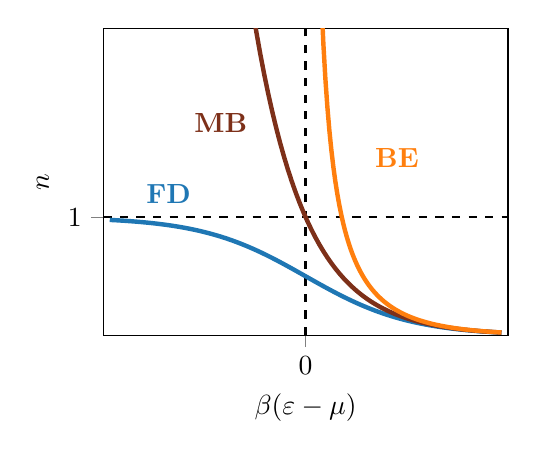
\begin{tikzpicture}

\definecolor{color0}{rgb}{0.12156862745098,0.466666666666667,0.705882352941177}
\definecolor{color1}{rgb}{1,0.498039215686275,0.0549019607843137}
\definecolor{color2}{rgb}{0.172549019607843,0.627450980392157,0.172549019607843}

\begin{axis}[
scale=0.75,
y = 2cm,
xmin=-3.1, xmax=3.1,
ymin=0, ymax=2.6,
tick align=outside,
tick pos=left,
ylabel = {$\expval{n}$},
xtick = {0},
ytick = {1},
xlabel = {$\beta(\varepsilon - \mu)$},
x grid style={white!69.01960784313725!black},
y grid style={white!69.01960784313725!black}
]

\node at (-2.1,1.2) {\color{color0}\textbf{FD}};
\node at (-1.3,1.8) {\color{Sepia!80}\textbf{MB}};
\node at (1.4,1.5) {\color{color1}\textbf{BE}};



\addplot [thick, black, dashed, forget plot]
table {%
0 0
0 2.6
};
\addplot [thick, black, dashed, forget plot]
table {%
-3.1 1
3.1  1
};
\addplot [ultra thick, color0, forget plot]
table {%
-3 0.977022630089974
-2.93939393939394 0.975259027362491
-2.87878787878788 0.973363751617231
-2.81818181818182 0.971327557243786
-2.75757575757576 0.969140641919771
-2.6969696969697 0.966792627904751
-2.63636363636364 0.964272545296714
-2.57575757575758 0.961568817814162
-2.51515151515152 0.958669251744938
-2.45454545454545 0.955561028785873
-2.39393939393939 0.952230703584588
-2.33333333333333 0.948664206884684
-2.27272727272727 0.944846855266537
-2.21212121212121 0.940763368565415
-2.15151515151515 0.936397896133564
-2.09090909090909 0.931734053189477
-2.03030303030303 0.926754968561019
-1.96969696969697 0.9214433451738
-1.90909090909091 0.915781534655735
-1.84848484848485 0.909751627415579
-1.78787878787879 0.903335559499269
-1.72727272727273 0.896515237424059
-1.66666666666667 0.889272682027632
-1.60606060606061 0.881590192138079
-1.54545454545455 0.873450528562205
-1.48484848484848 0.864837118496269
-1.42424242424242 0.855734279979351
-1.36363636363636 0.846127465432218
-1.3030303030303 0.836003522654966
-1.24242424242424 0.825350970901034
-1.18181818181818 0.814160288815684
-1.12121212121212 0.802424210143189
-1.06060606060606 0.790138022195814
-1 0.777299861174691
-0.939393939393939 0.763910997580872
-0.878787878787879 0.74997610420435
-0.818181818181818 0.73550349858496
-0.757575757575757 0.720505351459346
-0.696969696969697 0.704997852599438
-0.636363636363636 0.689001325661223
-0.575757575757576 0.672540284239115
-0.515151515151515 0.655643422286646
-0.454545454545455 0.638343533424372
-0.393939393939394 0.620677355392887
-0.333333333333333 0.602685337978492
-0.272727272727272 0.584411335070708
-0.212121212121212 0.56590222400902
-0.151515151515151 0.547207457925119
-0.0909090909090908 0.528378559257178
-0.0303030303030303 0.509468564870001
0.0303030303030303 0.490531435129999
0.0909090909090908 0.471621440742822
0.151515151515151 0.452792542074881
0.212121212121212 0.43409777599098
0.272727272727273 0.415588664929292
0.333333333333333 0.397314662021508
0.393939393939394 0.379322644607113
0.454545454545455 0.361656466575628
0.515151515151515 0.344356577713354
0.575757575757576 0.327459715760885
0.636363636363637 0.310998674338777
0.696969696969697 0.295002147400562
0.757575757575758 0.279494648540653
0.818181818181818 0.26449650141504
0.878787878787879 0.25002389579565
0.939393939393939 0.236089002419128
1 0.222700138825309
1.06060606060606 0.209861977804186
1.12121212121212 0.197575789856811
1.18181818181818 0.185839711184316
1.24242424242424 0.174649029098967
1.3030303030303 0.163996477345034
1.36363636363636 0.153872534567782
1.42424242424242 0.144265720020649
1.48484848484849 0.135162881503731
1.54545454545455 0.126549471437795
1.60606060606061 0.118409807861921
1.66666666666667 0.110727317972368
1.72727272727273 0.103484762575941
1.78787878787879 0.0966644405007311
1.84848484848485 0.090248372584421
1.90909090909091 0.0842184653442654
1.96969696969697 0.0785566548261996
2.03030303030303 0.0732450314389812
2.09090909090909 0.0682659468105229
2.15151515151515 0.0636021038664357
2.21212121212121 0.0592366314345846
2.27272727272727 0.0551531447334633
2.33333333333333 0.0513357931153162
2.39393939393939 0.0477692964154116
2.45454545454546 0.0444389712141272
2.51515151515152 0.0413307482550625
2.57575757575758 0.0384311821858377
2.63636363636364 0.0357274547032864
2.6969696969697 0.0332073720952487
2.75757575757576 0.0308593580802294
2.81818181818182 0.0286724427562142
2.87878787878788 0.0266362483827693
2.93939393939394 0.0247409726375094
3 0.0229773699100256
};
\addplot [ultra thick, Sepia!80, forget plot]
table {%
-3 42.5210820000628
-2.93939393939394 39.4187828284453
-2.87878787878788 36.5428245610929
-2.81818181818182 33.8766935730744
-2.75757575757576 31.4050810583992
-2.6969696969697 29.1137951275307
-2.63636363636364 26.9896793181859
-2.57575757575758 25.0205370515121
-2.51515151515152 23.1950615998711
-2.45454545454545 21.5027711641105
-2.39393939393939 19.9339486875376
-2.33333333333333 18.4795860610098
-2.27272727272727 17.1313323987719
-2.21212121212121 15.8814460880394
-2.15151515151515 14.7227503370014
-2.09090909090909 13.6485919659999
-2.03030303030303 12.6528032052669
-1.96969696969697 11.7296662798641
-1.90909090909091 10.8738805784721
-1.84848484848485 10.0805322175153
-1.78787878787879 9.34506582586009
-1.72727272727273 8.66325838807586
-1.66666666666667 8.03119499606725
-1.60606060606061 7.44524636984554
-1.54545454545455 6.90204801836367
-1.48484848484848 6.39848092075779
-1.42424242424242 5.93165361706764
-1.36363636363636 5.49888560560163
-1.3030303030303 5.09769195161484
-1.24242424242424 4.72576901892389
-1.18181818181818 4.38098124253003
-1.12121212121212 4.06134886629952
-1.06060606060606 3.76503657529169
-1 3.49034295746184
-0.939393939393939 3.2356907342287
-0.878787878787879 2.99961770381068
-0.818181818181818 2.78076834532806
-0.757575757575757 2.57788603546213
-0.696969696969697 2.38980583297983
-0.636363636363636 2.21544778969276
-0.575757575757576 2.05381074944258
-0.515151515151515 1.90396659950666
-0.454545454545455 1.76505494141602
-0.393939393939394 1.63627815058539
-0.333333333333333 1.51689679638821
-0.272727272727272 1.40622539637875
-0.212121212121212 1.30362848028224
-0.151515151515151 1.20851694115277
-0.0909090909090908 1.12034465274726
-0.0303030303030303 1.0386053336928
0.0303030303030303 0.96282964044144
0.0909090909090908 0.892582472320324
0.151515151515151 0.82746047320291
0.212121212121212 0.767089715455969
0.272727272727273 0.711123552863686
0.333333333333333 0.659240630200444
0.393939393939394 0.611143038023359
0.454545454545455 0.566554602089466
0.515151515151515 0.525219297575446
0.575757575757576 0.486899778994442
0.636363636363637 0.451376017368786
0.696969696969697 0.418444036833364
0.757575757575758 0.387914743415231
0.818181818181818 0.359612839264404
0.878787878787879 0.333375816101369
0.939393939393939 0.309053022101747
1 0.28650479686019
1.06060606060606 0.265601669466525
1.12121212121212 0.246223615089522
1.18181818181818 0.228259365799635
1.24242424242424 0.211605771673477
1.3030303030303 0.196167208511535
1.36363636363636 0.18185502876825
1.42424242424242 0.168587052541742
1.48484848484849 0.156287095700454
1.54545454545455 0.14488453243724
1.60606060606061 0.134313889739118
1.66666666666667 0.124514471444123
1.72727272727273 0.115430009726641
1.78787878787879 0.107008342010043
1.84848484848485 0.0992011114514831
1.90909090909091 0.0919634892790508
1.96969696969697 0.0852539173869474
2.03030303030303 0.0790338697106846
2.09090909090909 0.07326763101213
2.15151515151515 0.0679220918041915
2.21212121212121 0.0629665582376102
2.27272727272727 0.0583725758582377
2.33333333333333 0.0541137662228216
2.39393939393939 0.0501656754351527
2.45454545454546 0.0465056337328773
2.51515151515152 0.0431126253187255
2.57575757575758 0.0399671676887354
2.63636363636364 0.0370511997645778
2.6969696969697 0.0343479781876454
2.75757575757576 0.0318419811794293
2.81818181818182 0.0295188194161549
2.87878787878788 0.027365153405922
2.93939393939394 0.0253686168939336
3 0.0235177458560091
};
\addplot [ultra thick, color1, forget plot]
table {%
0 inf
0.0303030303030303 25.9031564901751
0.0606060606060606 12.7063125275225
0.0909090909090908 8.30946765952429
0.121212121212121 6.11262143428024
0.151515151515152 4.79577340081625
0.181818181818182 3.91892310939073
0.212121212121212 3.29349868322777
0.242424242424242 2.82521396167669
0.272727272727273 2.46168754813066
0.303030303030303 2.17149042937069
0.333333333333333 1.93462216633464
0.363636363636364 1.73774898964402
0.393939393939394 1.57163969732416
0.424242424242424 1.4297004536184
0.454545454545455 1.30709566838314
0.484848484848485 1.20019854680692
0.515151515151515 1.10623556284684
0.545454545454545 1.02304944160068
0.575757575757576 0.948936989425245
0.606060606060606 0.882535575087063
0.636363636363636 0.82274204493208
0.666666666666667 0.768653752156565
0.696969696969697 0.719524969798075
0.727272727272727 0.674734200525591
0.757575757575758 0.633759332122564
0.787878787878788 0.596158526358522
0.818181818181818 0.561555354812744
0.848484848484849 0.529627119909685
0.878787878787879 0.500095592319619
0.909090909090909 0.472719600903755
0.939393939393939 0.447289056885139
0.96969696969697 0.423620098506363
1 0.401551118493013
1.03030303030303 0.380939492566744
1.06060606060606 0.36165886879616
1.09090909090909 0.34359690873183
1.12121212121212 0.326653394851001
1.15151515151515 0.31073863683218
1.18181818181818 0.295772123021803
1.21212121212121 0.281681374182797
1.24242424242424 0.268400964987579
1.27272727272727 0.255871685296652
1.3030303030303 0.244039818465591
1.33333333333333 0.232856518060986
1.36363636363636 0.222277267675996
1.39393939393939 0.212261411198757
1.42424242424242 0.202771743039528
1.45454545454545 0.193774149571544
1.48484848484848 0.185237294468317
1.51515151515152 0.177132341790955
1.54545454545455 0.169432711643245
1.57575757575758 0.162113864009539
1.60606060606061 0.155153107052441
1.63636363636364 0.148529426698852
1.66666666666667 0.142223334804301
1.6969696969697 0.136216733572651
1.72727272727273 0.130492794234371
1.75757575757576 0.125035848261984
1.78787878787879 0.119831289634786
1.81818181818182 0.114865486863319
1.84848484848485 0.110125703653264
1.87878787878788 0.105600027233005
1.90909090909091 0.101277303493045
1.93939393939394 0.0971470781919676
1.96969696969697 0.0931995435754281
2 0.089425489833852
2.03030303030303 0.0858162608931738
2.06060606060606 0.0823637140924376
2.09090909090909 0.0790601833538513
2.12121212121212 0.0758984454959869
2.15151515151515 0.0728716893801999
2.18181818181818 0.0699734876148052
2.21212121212121 0.0671977705717541
2.24242424242424 0.0645388024970951
2.27272727272727 0.0619911595198503
2.3030303030303 0.0595497093845231
2.33333333333333 0.0572095927506321
2.36363636363636 0.0549662059187438
2.39393939393939 0.0528151848567227
2.42424242424242 0.0507523904125633
2.45454545454545 0.0487738946114011
2.48484848484848 0.0468759679443064
2.51515151515152 0.0450550675653817
2.54545454545455 0.0433078263216422
2.57575757575758 0.0416310425472794
2.60606060606061 0.0400216705602786
2.63636363636364 0.0384768118050715
2.66666666666667 0.0369937065900355
2.6969696969697 0.0355697263732544
2.72727272727273 0.034202366554107
2.75757575757576 0.0328892397319808
2.78787878787879 0.0316280693967816
2.81818181818182 0.0304166840189485
2.84848484848485 0.0292530115094396
2.87878787878788 0.0281350740226385
2.90909090909091 0.027060983077392
2.93939393939394 0.0260289349734317
2.96969696969697 0.0250372064822928
3 0.0240841507935291
};
\end{axis}

\end{tikzpicture}
	\vspace{0.5cm}
\end{wrapfigure}
Resulta entonces que, en el límite de densidades bajas o temperaturas altas, debe cumplirse \eqref{eq:lim_exp}, cuya forma es independiente de la estadística de que se trate bien sea la de Fermi-Dirac o la de Bose-Einstein.
Despreciando la unidad frente a $e^{\beta\varepsilon_r + \alpha}$ en \eqref{eq:sum_r_cas1_2}, en el límite señalado obtenemos para ambas estadísticas (figura adyacente).
\begin{equation}\label{eq:n_r_MB}
	\expval{n_r} = \exp[-\beta\varepsilon_r - \alpha]
\end{equation}

El parámetro $\alpha$ puede determinarse por la condición
\begin{equation}
	\expval{N} = \sum_r \expval{n_r} = \sum_r \exp[-\beta\varepsilon_r - \alpha] = e^{-\alpha} \sum_r e^{-\beta\varepsilon_r}
\end{equation}
de donde se puede despejar $e^{\alpha}$ e introducirse en \eqref{eq:n_r_MB}, resultando
\begin{equation}
	\expval{n_r} = \expval{N} \frac{e^{-\beta\varepsilon_r}}{\sum_r e^{-\beta\varepsilon_r}}
\end{equation}
siendo $\expval{N} = N$ en el caso de un sistema cerrado.

En el mismo límite y utilizando la aproximación
$$\ln(1+x) \approx x \qquad x \ll 1$$
obtenemos para la función de partición generalizada
\begin{equation}
	\ln Q = \pm \sum_r \ln(1 \pm e^{-\beta\varepsilon_r}) = \sum_r e^{\beta\varepsilon_r}
\end{equation}

Sustituyendo en esta expresión el valor de $e^{-\alpha}$ que obtuvimos antes resulta
\begin{equation}
	\ln Q = \expval{N}
\end{equation}
que es el mismo resultado que se obtiene mediante la Mecánica Estadística Clásica.

\section{Gas ideal monoatómico}
En general, definimos la función de partición por partículas de un gas ideal en el límite clásico como
\begin{equation}\label{eq:zeta_lim}
	\zeta = e^{-\beta\varepsilon_r}
\end{equation}

En el caso de un gas ideal monoatómico (sin grados internos de libertad) el estudio de los estados cuánticos accesibles a un átomo es equivalente al estudio de los estados estacionarios de una partícula puntual encerrada en un volumen $V$ y que, como ya sabemos, vienen caracterizados por tres números cuánticos $n_x$, $n_y$ y $n_z$ y cuya energía asociada a un estado es
\begin{equation}
\varepsilon_r \equiv \frac{\hbar^2 \pi^2}{2m} \left[\left( \frac{n_x}{L_x} \right)^2 + \left( \frac{n_y}{L_y} \right)^2 + \left( \frac{n_z}{L_z} \right)^2 \right] 
\end{equation}

Teniendo en cuenta que sumar para todos los estados de una partícula es equivalente a sumar sobre todos los valores posibles de $n_x$, $n_y$ y $n_z$ que son enteros positivos, resulta
\begin{align}\label{eq:z_gen}
	\zeta &= \sum_{n_x=1}^{\infty} \sum_{n_y=1}^{\infty} \sum_{n_z=1}^{\infty} \exp \left\lbrace - \beta \frac{\hbar^2 \pi^2}{2m} \left[\left( \frac{n_x}{L_x} \right)^2 + \left( \frac{n_y}{L_y} \right)^2 + \left( \frac{n_z}{L_z} \right)^2 \right]  \right\rbrace \nonumber \\
		&= \left\lbrace \sum_{n_x=1}^{\infty} \exp \left[ -\beta \frac{\hbar^2 \pi^2}{2m} \left( \frac{n_x}{L_x} \right)^2 \right] \right\rbrace \left\lbrace \sum_{n_y=1}^{\infty} \exp \left[ -\beta \frac{\hbar^2 \pi^2}{2m} \left( \frac{n_y}{L_y} \right)^2 \right] \right\rbrace \times \\
		&\times \left\lbrace \sum_{n_z=1}^{\infty} \exp \left[ -\beta \frac{\hbar^2 \pi^2}{2m} \left( \frac{n_z}{L_z} \right)^2 \right] \right\rbrace \nonumber
\end{align}
y vamos a ver cómo puede evaluarse cada una de las sumas indicadas.
Consideremos, por ejemplo, la primera de ellas y calculemos la variación del exponente al pasar de un sumando al siguiente.

Resulta entonces, que la diferencia entre dos sumandos consecutivos de cada una de las sumas \eqref{eq:z_gen} es muy pequeña frente al valor de cada uno de los sumandos, pues
\begin{equation}
	\abs{\frac{\exp \left[ -\beta \frac{\hbar^2 \pi^2}{2m} \left( \frac{n_x + 1}{L_x} \right)^2 \right] - \exp \left[ -\beta \frac{\hbar^2 \pi^2}{2m} \left( \frac{n_x}{L_x} \right)^2 \right]}{\exp \left[ -\beta \frac{\hbar^2 \pi^2}{2m} \left( \frac{n_x + 1}{L_x} \right)^2 \right]}} = \abs{1 - \exp \left[ -\beta \frac{\hbar^2 \pi^2}{2m} \left( \frac{2n_x + 1}{L_x} \right)^2 \right]} \ll 1
\end{equation}

La consecuencia es que las sumas pueden sustituirse por integrales, como ya hemos hecho repetidamente, o sea, que podemos escribir
\begin{equation}
	\sum_{n_x=1}^{\infty} \exp \left[ -\beta \frac{\hbar^2 \pi^2}{2m} \left( \frac{n_x}{L_x} \right)^2 \right] = \int_{0}^{\infty} \exp \left[ -\beta \frac{\hbar^2 \pi^2}{2m} \left( \frac{n_x}{L_x} \right)^2 \right] = \frac{1}{2}\sqrt{\frac{2\pi m L_x^2}{\beta \hbar^2 \pi^2}}
\end{equation}
y análogamente para las sumas respecto de $n_y$ y $n_z$.
En resumen, sustituyendo estas expresiones en \eqref{eq:z_gen} obtenemos la función de partición de una partícula en el límite clásico
\begin{equation}
	\zeta = \frac{V}{(2\pi\hbar)^3}(2\pi m k_B T)^{3/2}= \frac{V}{h^3}(2\pi m k_B T)^{3/2}
\end{equation}
donde hemos introducido el volumen $V = L_x L_y L_z$ y hemos escrito $h = \hbar 2 \pi$. Con este resultado llegamos también a Q
\begin{equation}
	Q = \frac{\zeta^N}{N!} = \frac{V^N}{h^{3N}N!}(2\pi m k_B T)^{3N/2} = \frac{V^N}{N!} \left[ \frac{2\pi m k_B T}{h^2}\right] ^{\frac{3N}{2}}
\end{equation}

\section{Número de estados estacionarios}

El problema que vamos a resolver ahora es el siguiente: dado un valor de la energía
$\varepsilon$, ¿cuántos estados estacionarios corresponden a ese valor? 
El problema consiste en encontrar todos los valores posibles de $n_x$, $n_y$ y $n_z$ que satisfacen la relación dada.
Así planteado el problemas es de difícil resolución general; sin embargo, nosotros vamos a estar siempre interesados en volúmenes macroscópicos, de forma que $L_x$, $L_y$ y $L_z$ van a ser muy grandes y en consecuencia los valores de la energía van a estar muy próximos entre sí, permitiéndonos incluso hablar de una distribución continua de energía desde un punto de vista matemático.
Por ello, vamos a cambiar nuestra pregunta formulándola del modo siguiente: ¿cuántos estados estacionarios pueden encontrarse con una energía comprendida entre $\varepsilon$ y $\varepsilon + d\varepsilon$?

Consideremos los estados que existen en una componente $p_x$ de la cantidad de
movimiento cuyo valor absoluto esté comprendido entre $\abs{p_x}$ y $\abs{p_x} + d\abs{p_x}$, para valores
dados de $n_y$ y $n_z$.
Evidentemente dicho número vendrá dado por
\begin{equation}
	D(\abs{p_x}) d\abs{p_x} = \Delta n_x
\end{equation}
siendo $\Delta n_x$ el número de valores enteros de $n_x$ para los que $\abs{p_x}$ está dentro del intervalo citado.
Ahora bien, podemos calcular la expresión de $p_x$ y así
\begin{equation}
	p_x = \pm\hbar\frac{n_x\pi}{L_x} \Rightarrow \Delta n_x = \frac{L_x}{n_x\pi}d\abs{p_x}
\end{equation}
luego
\begin{equation}
	D(\abs{p_x}) d\abs{p_x} = \frac{L_x}{\hbar\pi}d\abs{p_x}
\end{equation}

Es evidente entonces que el número de estados correspondientes a cantidades de movimiento con componentes cuyo valor absoluto está comprendido entre $\abs{p_x}$ y $\abs{p_x} + d\abs{p_x}$, $\abs{p_y}$ y $\abs{p_y} + d\abs{p_y}$ y $\abs{p_z}$ y $\abs{p_z} + d\abs{p_z}$ será
\begin{equation}
	D(\abs{p_x}, \abs{p_y}, \abs{p_z}) \, d\abs{p_x} d\abs{p_y} d\abs{p_z}= \frac{L_xL_yL_z}{(\hbar\pi)^3} d\abs{p_x} d\abs{p_y} d\abs{p_z}
\end{equation}
es decir
\begin{equation}
	D(\abs{p_x}, \abs{p_y}, \abs{p_z}) \, d\abs{p_x} d\abs{p_y} d\abs{p_z}= \frac{V}{(\hbar\pi)^3} d\abs{p_x} d\abs{p_y} d\abs{p_z}
\end{equation}

Pasemos ahora a calcular el número de estados con cantidad de movimiento \textbf{p} con un módulo comprendido entre $p$ y $p+dp$.
De la figura se deduce que\footnote{El volumen de la corteza esférica de anchura $dp$ es $\sfrac{4}{3}\pi[(p + dp)^3 - p^3]=4\pi p^2 dp + \order{(dp)^2}$. El factor 8 proviene de que solo hay que elegir un octante.}
\begin{equation}
	D(p)dp = D(\abs{p_x}, \abs{p_y}, \abs{p_z}) \frac{4\pi p^2 dp}{8}
\end{equation}
o sea
\begin{equation}
	D(p)dp = \frac{V}{(2\hbar\pi)^3}4\pi p^2 dp = \frac{4\pi V}{h^3} p^2 dp
\end{equation}

De esta distribución de densidades para $p$ ya es fácil pasar a la distribución para la energía.
Del hecho de que $E = p^2/2m$ tenemos
\begin{equation}
	D(\varepsilon) d\varepsilon = D(p)\abs{\frac{dp}{d\varepsilon}}d\varepsilon = D(p) \abs{\frac{d\varepsilon}{dp}}^{-1} d\varepsilon
\end{equation}
o sea
\begin{equation}\label{eq:D_vareps}
	D(\varepsilon) d\varepsilon = \frac{4\pi V\sqrt{2m^3}}{h^3} d\varepsilon
\end{equation}
con lo que hemos obtenido la distribución buscada.


